\p
یک شکل را در نظر بگیرید که از n دایره تشکیل شده است و بین برخی از دایره‌ها پاره خطی رسم شده باشد، می‌خواهیم در دایره‌های این شکل برچسب‌های 1 تا n را بنویسیم 
به طوری که اعداد واقع در هیچ دو دایره ای برابر نباشند. دو روش برچسب‌گذاری را متمایز گوییم هرگاه دو عدد وجود داشته باشند که دایره‌های شامل این دو عدد در یکی مجاور و در دیگری غیر مجاور باشند.
مثلا برچسب‌گذاری‌های زیر یکسانند:

\begin{figure}[h]
\centering
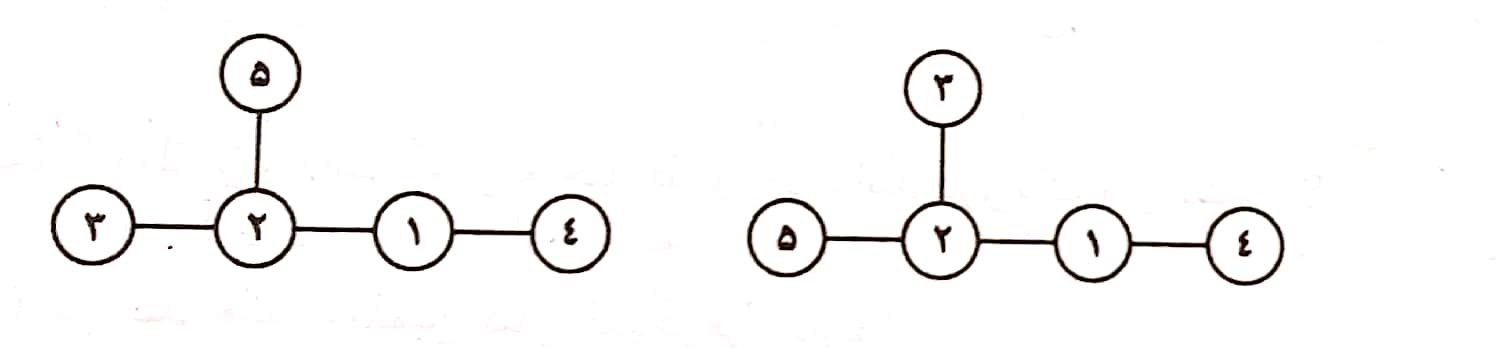
\includegraphics[scale = 0.18]{./figure B.jpg}
\label{fig:mesh2}
\end{figure}

برای هر یک از شکل‌های زیر تعداد راه‌های برچسب گذاری را بیابید:

\begin{figure}[h]
\centering
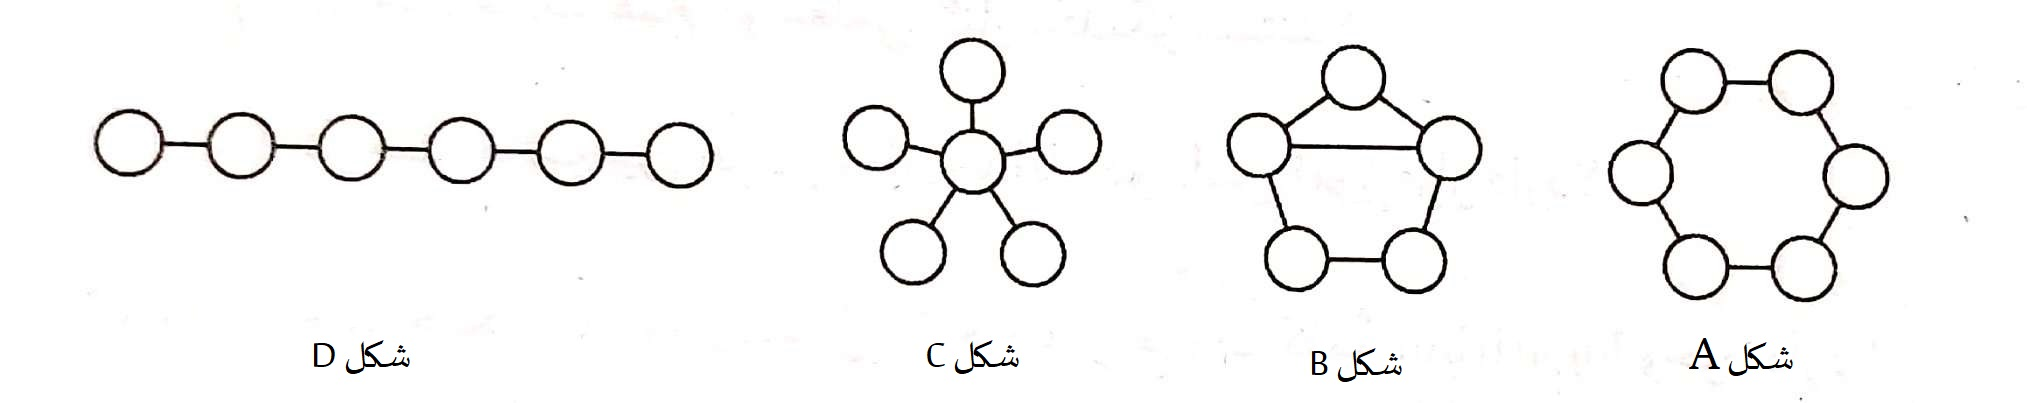
\includegraphics[scale = 0.16]{./figure C.JPEG}
\label{fig:mesh3}
\end{figure}